\documentclass[12pt,]{article}
\usepackage{lmodern}
\usepackage{amssymb,amsmath}
\usepackage{ifxetex,ifluatex}
\usepackage{fixltx2e} % provides \textsubscript
\ifnum 0\ifxetex 1\fi\ifluatex 1\fi=0 % if pdftex
  \usepackage[T1]{fontenc}
  \usepackage[utf8]{inputenc}
\else % if luatex or xelatex
  \ifxetex
    \usepackage{mathspec}
  \else
    \usepackage{fontspec}
  \fi
  \defaultfontfeatures{Ligatures=TeX,Scale=MatchLowercase}
\fi
% use upquote if available, for straight quotes in verbatim environments
\IfFileExists{upquote.sty}{\usepackage{upquote}}{}
% use microtype if available
\IfFileExists{microtype.sty}{%
\usepackage{microtype}
\UseMicrotypeSet[protrusion]{basicmath} % disable protrusion for tt fonts
}{}
\usepackage[margin=1in]{geometry}
\usepackage{hyperref}
\PassOptionsToPackage{usenames,dvipsnames}{color} % color is loaded by hyperref
\hypersetup{unicode=true,
            pdftitle={Dashboards project},
            pdfauthor={Richard White},
            colorlinks=true,
            linkcolor=Maroon,
            citecolor=Blue,
            urlcolor=Blue,
            breaklinks=true}
\urlstyle{same}  % don't use monospace font for urls
\usepackage{natbib}
\bibliographystyle{apalike}
\usepackage{longtable,booktabs}
\usepackage{graphicx,grffile}
\makeatletter
\def\maxwidth{\ifdim\Gin@nat@width>\linewidth\linewidth\else\Gin@nat@width\fi}
\def\maxheight{\ifdim\Gin@nat@height>\textheight\textheight\else\Gin@nat@height\fi}
\makeatother
% Scale images if necessary, so that they will not overflow the page
% margins by default, and it is still possible to overwrite the defaults
% using explicit options in \includegraphics[width, height, ...]{}
\setkeys{Gin}{width=\maxwidth,height=\maxheight,keepaspectratio}
\IfFileExists{parskip.sty}{%
\usepackage{parskip}
}{% else
\setlength{\parindent}{0pt}
\setlength{\parskip}{6pt plus 2pt minus 1pt}
}
\setlength{\emergencystretch}{3em}  % prevent overfull lines
\providecommand{\tightlist}{%
  \setlength{\itemsep}{0pt}\setlength{\parskip}{0pt}}
\setcounter{secnumdepth}{5}
% Redefines (sub)paragraphs to behave more like sections
\ifx\paragraph\undefined\else
\let\oldparagraph\paragraph
\renewcommand{\paragraph}[1]{\oldparagraph{#1}\mbox{}}
\fi
\ifx\subparagraph\undefined\else
\let\oldsubparagraph\subparagraph
\renewcommand{\subparagraph}[1]{\oldsubparagraph{#1}\mbox{}}
\fi

%%% Use protect on footnotes to avoid problems with footnotes in titles
\let\rmarkdownfootnote\footnote%
\def\footnote{\protect\rmarkdownfootnote}

%%% Change title format to be more compact
\usepackage{titling}

% Create subtitle command for use in maketitle
\newcommand{\subtitle}[1]{
  \posttitle{
    \begin{center}\large#1\end{center}
    }
}

\setlength{\droptitle}{-2em}

  \title{Dashboards project}
    \pretitle{\vspace{\droptitle}\centering\huge}
  \posttitle{\par}
    \author{Richard White}
    \preauthor{\centering\large\emph}
  \postauthor{\par}
      \predate{\centering\large\emph}
  \postdate{\par}
    \date{2018-11-05}

\usepackage{booktabs}

\begin{document}
\maketitle

{
\hypersetup{linkcolor=black}
\setcounter{tocdepth}{2}
\tableofcontents
}
\listoftables
\listoffigures
\section*{Preface}\label{preface}
\addcontentsline{toc}{section}{Preface}

The dashboards project is a project at FHI concerned with running
automated analyses on data. An automated analysis is any analysis that:

\begin{enumerate}
\def\labelenumi{\arabic{enumi}.}
\tightlist
\item
  Will be repeated multiple times in the future
\item
  Always has an input dataset with consistent file structure
\item
  Always has the same expected output (e.g.~tables, graphs, reports)
\end{enumerate}

\section{Introduction}\label{introduction}

\subsection{Executive summary}\label{executive-summary}

The dashboards project is a project at FHI concerned with running
automated analyses on data.

In principle, the dashboards project is split up into two parts:

\begin{enumerate}
\def\labelenumi{\arabic{enumi}.}
\tightlist
\item
  The umbrella infrastructure (i.e.~Docker containers, continuous
  integration, chron jobs, etc.)
\item
  The R package for each automated analysis
\end{enumerate}

\subsection{What is an automated
analysis?}\label{what-is-an-automated-analysis}

An automated analysis is any analysis that:

\begin{enumerate}
\def\labelenumi{\arabic{enumi}.}
\tightlist
\item
  Will be repeated multiple times in the future
\item
  Always has an input dataset with consistent file structure
\item
  Always has the same expected output (e.g.~tables, graphs, reports)
\end{enumerate}

\subsection{Why not have one project for each automated
analysis?}\label{why-not-have-one-project-for-each-automated-analysis}

Automated analyses have a lot of code and infrastructure in common.

Automated analyses:

\begin{enumerate}
\def\labelenumi{\arabic{enumi}.}
\tightlist
\item
  Need their code to be tested via unit testing to ensure the results
  are correct
\item
  Need their code to be tested via integration testing to ensure
  everything runs
\item
  Need to be run at certain times
\item
  Need to be able to send emails notifying people that the analyses have
  finished running
\item
  Need to make their results accessible to the relevant people
\end{enumerate}

By combining them all in one umbrella project we can force everyone to
use the same infrastructure and coding principles, so we:

\begin{enumerate}
\def\labelenumi{\arabic{enumi}.}
\tightlist
\item
  Only need to solve a problem once
\item
  Only need to maintain one system
\item
  Can easily work on multiple projects, as we all speak the same
  language
\end{enumerate}

\subsection{Important repositories}\label{important-repositories}

\subsubsection{Infrastructure}\label{infrastructure}

\url{https://github.com/raubreywhite/dashboards_control/} (private)

This contains the Dockerfiles, cronfiles, all bash scripts, etc.

\url{http://github.com/raubreywhite/docker/}

This contains the base analysis Dockerfile

\url{https://rocker-project.org}

\url{https://folkehelseinstituttet.github.io/fhi/}

This is an R package that contains helper functions.

\subsubsection{Automated analyses R
packages}\label{automated-analyses-r-packages}

\url{https://folkehelseinstituttet.github.io/dashboards_sykdomspuls/}

\url{https://folkehelseinstituttet.github.io/dashboards_normomo/}

\url{https://folkehelseinstituttet.github.io/dashboards_sykdomspuls_pdf/}

\url{https://folkehelseinstituttet.github.io/dashboards_noispiah/}

\url{https://folkehelseinstituttet.github.io/dashboards_sykdomspuls_log/}

\section{Umbrella Infrastructure}\label{umbrella-infrastructure}

\subsection{Physical Hardware and
Subscriptions}\label{physical-hardware-and-subscriptions}

\begin{itemize}
\tightlist
\item
  One Github organization
  (\url{http://github.com/folkehelseinstituttet/})
\item
  One Github team
  (\url{https://github.com/orgs/folkehelseinstituttet/teams/dashboards})
\item
  One \href{https://github.com/eddelbuettel/drat}{drat} repository
  (\url{https://folkehelseinstituttet.github.io/drat/})
\item
  One travis-ci.org account
  (\url{http://travis-ci.org/folkehelseinstituttet})
\item
  One travis-ci.com account
  (\url{http://travis-ci.com/folkehelseinstituttet})
\item
  One Docker hub account (\url{http://hub.docker.com/u/raw996/})
\item
  At least three computers:

  \begin{enumerate}
  \def\labelenumi{\arabic{enumi}.}
  \tightlist
  \item
    Production linux computer \texttt{smhb}
  \item
    Testing linux computer \texttt{linux}
  \item
    Development linux computers (1 per person)
  \end{enumerate}
\end{itemize}

\subsubsection{Requirements - smhb}\label{requirements---smhb}

\begin{itemize}
\tightlist
\item
  Git
\item
  Docker Engine - Community
  (\url{https://www.docker.com/products/docker-engine})
\end{itemize}

\subsubsection{Requirements - linux}\label{requirements---linux}

\begin{itemize}
\tightlist
\item
  Git
\item
  Docker Engine - Community
  (\url{https://www.docker.com/products/docker-engine})
\item
  Jenkins installed via a Docker container (\url{http://jenkins.io})
\end{itemize}

\subsubsection{Requirements - dev}\label{requirements---dev}

\begin{itemize}
\tightlist
\item
  Git
\item
  Docker Engine - Community
  (\url{https://www.docker.com/products/docker-engine})
\end{itemize}

\subsection{Configuration, Scripts,
etc.}\label{configuration-scripts-etc.}

Most of the bash scripts, Docker files, passwords, etc. are all hosted
at the private Github repository
\href{https://github.com/raubreywhite/dashboards_control}{raubreywhite/dashboards\_control}.

\begin{verbatim}
- $DASHBOARDS_FOLDER/dashboards_control/
  |-- bin/
    |-- dev_down.sh
    |-- dev_up.sh
    |-- docker_build.sh
    |-- docker_login.sh
    |-- docker_push_test_to_prod.sh
    |-- prod_down.sh
    |-- prod_up.sh
    |-- prod_update.sh
    |-- public.sh
    |-- test_noispiah.sh
    |-- test_normomo.sh
    |-- test_sykdomspuls_log.sh
    |-- test_sykdomspuls_pdf.sh
    |-- test_sykdomspuls.sh
  |-- infrastructure/
    |-- dashboards_nginx/
    |-- dashboards_r/
      |-- add_autofs.sh
      |-- add_cron.sh
      |-- auto.mounts
      |-- crontab
      |-- Dockerfile
      |-- emails_sykdomspuls_alert_test.xlsx
      |-- emails_sykdomspuls_alert.xlsx
      |-- emails.xlsx
      |-- httr-oauth_2017_09_17
      |-- mail.json
      |-- repo-key
      |-- secret.sh
    |-- dashboards_shiny/
    |-- docker-compose-api.yml
    |-- docker-compose-dev.yml
    |-- docker-compose-prod.yml
    |-- docker-compose-test.yml
\end{verbatim}

\subsubsection{\$DASHBOARDS\_FOLDER/dashboards\_control/bin/dev\_down.sh}\label{dashboards_folderdashboards_controlbindev_down.sh}

Dev script to shut down docker-compose

\subsubsection{\$DASHBOARDS\_FOLDER/dashboards\_control/bin/dev\_up.sh}\label{dashboards_folderdashboards_controlbindev_up.sh}

Dev script to start docker-compose

\subsubsection{\$DASHBOARDS\_FOLDER/dashboards\_control/bin/docker\_build.sh}\label{dashboards_folderdashboards_controlbindocker_build.sh}

Builds all relevant Docker containers

\subsubsection{\$DASHBOARDS\_FOLDER/dashboards\_control/bin/docker\_login.sh}\label{dashboards_folderdashboards_controlbindocker_login.sh}

Logs in to docker-hub

\subsubsection{\$DASHBOARDS\_FOLDER/dashboards\_control/bin/docker\_push\_test\_to\_prod.sh}\label{dashboards_folderdashboards_controlbindocker_push_test_to_prod.sh}

Retags `test' Docker containers to `production' and pushs them to
docker-hub

\subsubsection{\$DASHBOARDS\_FOLDER/dashboards\_control/bin/prod\_down.sh}\label{dashboards_folderdashboards_controlbinprod_down.sh}

Only to be used on the production computer \texttt{smhb}. This bash
script stops the docker-compose.

Note: This script is not used.

\subsubsection{\$DASHBOARDS\_FOLDER/dashboards\_control/bin/prod\_up.sh}\label{dashboards_folderdashboards_controlbinprod_up.sh}

Only to be used on the production computer \texttt{smhb}. This bash
script starts up the docker-compose.

Note: This script is not used.

\subsubsection{\$DASHBOARDS\_FOLDER/dashboards\_control/bin/prod\_update.sh}\label{dashboards_folderdashboards_controlbinprod_update.sh}

Only to be used on the production computer \texttt{smhb}. This bash
script:

\begin{enumerate}
\def\labelenumi{\arabic{enumi}.}
\tightlist
\item
  Removes unused Docker container/images (important so we don't run out
  of space)
\item
  Runs some scripts required for network access
\item
  Pulls the latest version of
  \href{https://github.com/raubreywhite/dashboards_control}{raubreywhite/dashboards\_control}
\item
  Stops the
  \href{https://github.com/raubreywhite/dashboards_control/blob/master/infrastructure/docker-compose-prod.yml}{docker-compose-prod.yml}
\item
  Pulls the latest production images for:

  \begin{itemize}
  \tightlist
  \item
    \href{https://github.com/raubreywhite/dashboards_control/blob/master/infrastructure/dashboards_r/Dockerfile}{raw996/dashboards\_r:production}
  \item
    \href{https://github.com/raubreywhite/dashboards_control/blob/master/infrastructure/dashboards_nginx/Dockerfile}{raw996/dashboards\_nginx:production}
  \item
    \href{https://github.com/raubreywhite/dashboards_control/blob/master/infrastructure/dashboards_shiny/Dockerfile}{raw996/dashboards\_shiny:production}
  \end{itemize}
\item
  Starts the
  \href{https://github.com/raubreywhite/dashboards_control/blob/master/infrastructure/docker-compose-prod.yml}{docker-compose-prod.yml}
\end{enumerate}

\subsubsection{\$DASHBOARDS\_FOLDER/dashboards\_control/bin/public.sh}\label{dashboards_folderdashboards_controlbinpublic.sh}

Lists a bunch of environmental variables

\subsubsection{\$DASHBOARDS\_FOLDER/dashboards\_control/bin/test\_noispiah.sh}\label{dashboards_folderdashboards_controlbintest_noispiah.sh}

Runs \texttt{/r/noispiah/src/RunTest.R} inside
\href{https://github.com/raubreywhite/dashboards_control/blob/master/infrastructure/dashboards_r/Dockerfile}{raw996/dashboards\_r:test}

Note: This script is generally only run by \texttt{Jenkins} on
\texttt{linux} as the integration testing for
\href{https://folkehelseinstituttet.github.io/dashboards_noispiah/}{noispiah}.

\subsubsection{\$DASHBOARDS\_FOLDER/dashboards\_control/bin/test\_normomo.sh}\label{dashboards_folderdashboards_controlbintest_normomo.sh}

Runs \texttt{/r/normomo/src/RunTest.R} inside
\href{https://github.com/raubreywhite/dashboards_control/blob/master/infrastructure/dashboards_r/Dockerfile}{raw996/dashboards\_r:test}

Note: This script is generally only run by \texttt{Jenkins} on
\texttt{linux} as the integration testing for
\href{https://folkehelseinstituttet.github.io/dashboards_normomo/}{normomo}.

\subsubsection{\$DASHBOARDS\_FOLDER/dashboards\_control/bin/test\_sykdomspuls\_log.sh}\label{dashboards_folderdashboards_controlbintest_sykdomspuls_log.sh}

Runs \texttt{/r/sykdomspulslog/src/RunTest.R} inside
\href{https://github.com/raubreywhite/dashboards_control/blob/master/infrastructure/dashboards_r/Dockerfile}{raw996/dashboards\_r:test}

Note: This script is generally only run by \texttt{Jenkins} on
\texttt{linux} as the integration testing for
\href{https://folkehelseinstituttet.github.io/dashboards_sykdomspuls_log/}{sykdomspuls\_log}.

\subsubsection{\$DASHBOARDS\_FOLDER/dashboards\_control/bin/test\_sykdomspuls\_pdf.sh}\label{dashboards_folderdashboards_controlbintest_sykdomspuls_pdf.sh}

Runs \texttt{/r/sykdomspulspdf/src/RunTest.R} inside
\href{https://github.com/raubreywhite/dashboards_control/blob/master/infrastructure/dashboards_r/Dockerfile}{raw996/dashboards\_r:test}

Note: This script is generally only run by \texttt{Jenkins} on
\texttt{linux} as the integration testing for
\href{https://folkehelseinstituttet.github.io/dashboards_sykdomspuls_pdf/}{sykdomspuls\_pdf}.

\subsubsection{\$DASHBOARDS\_FOLDER/dashboards\_control/bin/test\_sykdomspuls.sh}\label{dashboards_folderdashboards_controlbintest_sykdomspuls.sh}

Runs \texttt{/r/sykdomspuls/src/RunTest.R} inside
\href{https://github.com/raubreywhite/dashboards_control/blob/master/infrastructure/dashboards_r/Dockerfile}{raw996/dashboards\_r:test}

Note: This script is generally only run by \texttt{Jenkins} on
\texttt{linux} as the integration testing for
\href{https://folkehelseinstituttet.github.io/dashboards_sykdomspuls/}{sykdomspuls}.

\subsubsection{\$DASHBOARDS\_FOLDER/dashboards\_control/infrastructure/dashboards\_r/add\_autofs.sh}\label{dashboards_folderdashboards_controlinfrastructuredashboards_radd_autofs.sh}

See \protect\hypertarget{autofs}{}{autofs}.

\subsubsection{\$DASHBOARDS\_FOLDER/dashboards\_control/infrastructure/dashboards\_r/add\_cron.sh}\label{dashboards_folderdashboards_controlinfrastructuredashboards_radd_cron.sh}

See \protect\hypertarget{cron}{}{cron}.

\subsubsection{\$DASHBOARDS\_FOLDER/dashboards\_control/infrastructure/dashboards\_r/auto.mounts}\label{dashboards_folderdashboards_controlinfrastructuredashboards_rauto.mounts}

See \protect\hypertarget{autofs}{}{autofs}.

\subsubsection{\$DASHBOARDS\_FOLDER/dashboards\_control/infrastructure/dashboards\_r/crontab}\label{dashboards_folderdashboards_controlinfrastructuredashboards_rcrontab}

See \protect\hypertarget{cron}{}{cron}.

\subsubsection{\$DASHBOARDS\_FOLDER/dashboards\_control/infrastructure/dashboards\_r/Dockerfile}\label{dashboards_folderdashboards_controlinfrastructuredashboards_rdockerfile}

See \protect\hypertarget{analysisdocker}{}{here}.

\subsubsection{\$DASHBOARDS\_FOLDER/dashboards\_control/infrastructure/dashboards\_r/emails\_sykdomspuls\_alert\_test.xlsx}\label{dashboards_folderdashboards_controlinfrastructuredashboards_remails_sykdomspuls_alert_test.xlsx}

A list of email addresses used in
\href{https://folkehelseinstituttet.github.io/dashboards_sykdomspuls/}{sykdomspuls}.

\subsubsection{\$DASHBOARDS\_FOLDER/dashboards\_control/infrastructure/dashboards\_r/emails\_sykdomspuls\_alert.xlsx}\label{dashboards_folderdashboards_controlinfrastructuredashboards_remails_sykdomspuls_alert.xlsx}

A list of email addresses used in
\href{https://folkehelseinstituttet.github.io/dashboards_sykdomspuls/}{sykdomspuls}.

\subsubsection{\$DASHBOARDS\_FOLDER/dashboards\_control/infrastructure/dashboards\_r/emails.xlsx}\label{dashboards_folderdashboards_controlinfrastructuredashboards_remails.xlsx}

A list of email addresses used in many projects.

\subsubsection{\$DASHBOARDS\_FOLDER/dashboards\_control/infrastructure/dashboards\_r/httr-oauth\_2017\_09\_17}\label{httroauth}

The authorization file for the
\href{mailto:dashboardsfhi@gmail.com}{\nolinkurl{dashboardsfhi@gmail.com}}.
This probably needs to be refreshed every year??

\subsubsection{\$DASHBOARDS\_FOLDER/dashboards\_control/infrastructure/dashboards\_r/mail.json}\label{dashboards_folderdashboards_controlinfrastructuredashboards_rmail.json}

Related to \protect\hypertarget{httroauth}{}{httr-oauth}.

\subsubsection{\$DASHBOARDS\_FOLDER/dashboards\_control/infrastructure/dashboards\_r/repo-key}\label{dashboards_folderdashboards_controlinfrastructuredashboards_rrepo-key}

The repo-key for downloading the private
\href{https://github.com/raubreywhite/dashboards_control}{raubreywhite/dashboards\_control}
repository.

\subsubsection{\$DASHBOARDS\_FOLDER/dashboards\_control/infrastructure/dashboards\_r/secret.sh}\label{dashboards_folderdashboards_controlinfrastructuredashboards_rsecret.sh}

Passwords.

\subsubsection{\$DASHBOARDS\_FOLDER/dashboards\_control/infrastructure/docker-compose-api.yml}\label{dashboards_folderdashboards_controlinfrastructuredocker-compose-api.yml}

Docker-compose file used for testing the
\href{https://github.com/folkehelseinstituttet/dashboards_sykdomspuls/blob/master/inst/src/RunAPI.R}{API}.

\subsubsection{\$DASHBOARDS\_FOLDER/dashboards\_control/infrastructure/docker-compose-dev.yml}\label{dashboards_folderdashboards_controlinfrastructuredocker-compose-dev.yml}

Docker-compose file used for development.

\subsubsection{\$DASHBOARDS\_FOLDER/dashboards\_control/infrastructure/docker-compose-prod.yml}\label{dashboards_folderdashboards_controlinfrastructuredocker-compose-prod.yml}

Docker-compose file used for the production computer.

\subsubsection{\$DASHBOARDS\_FOLDER/dashboards\_control/infrastructure/docker-compose-test.yml}\label{dashboards_folderdashboards_controlinfrastructuredocker-compose-test.yml}

Docker-compose file used for integration testing of \texttt{Jenkins} on
\texttt{linux}.

\subsection{Analysis Docker Image}\label{analysisdocker}

\subsubsection{Images}\label{images}

Our analysis Docker images are based off the
\href{https://rocker-project.org}{rocker} images. More specifically, the
\href{https://hub.docker.com/r/rocker/verse/}{rocker/verse:3.5.0} image.

This Docker image is then expanded upon by a separate Dockerfile
\href{https://github.com/raubreywhite/docker/blob/master/dhadley/Dockerfile}{raw996/dhadley}.
This Docker image is automatically rebuilt by \texttt{Jenkins} on
\texttt{linux} whenever the repository is updated. The resultant Docker
image is pushed to
\href{https://hub.docker.com/r/raw996/dhadley/}{raw996/dhadley:3.5.0}.
This image is a general-purpose analysis image, with no sensitive
information in it.

This Docker image is then expanded upon by a separate Dockerfile
\href{https://github.com/raubreywhite/dashboards_control/blob/master/infrastructure/dashboards_r/Dockerfile}{raw996/dashboards\_r}.
This Docker image is automatically rebuilt by \texttt{Jenkins} on
\texttt{linux} whenever the repository is updated. The resultant Docker
image is locally tagged as \texttt{raw996/dashboards\_r:test} and then a
number of integration tests are performed on it. If the integration
tests are passed, then the Docker image is retagged and pushed to
\href{https://hub.docker.com/r/raw996/dashboards_r/}{raw996/dashboards\_r:production}.
This image is private as it contains passwords and email addresses.

\subsubsection{File Structure}\label{file-structure}

Inside \texttt{raw996/dashboards\_r} we have the following file
structure:

\begin{verbatim}
/data_raw/
  |-- normomo/
  |-- noispiah/
  |-- sykdomspuls/
  |-- sykdomspuls_pdf/
  |-- sykdomspuls_log/
/data_clean/
  |-- normomo/
  |-- noispiah/
  |-- sykdomspuls/
  |-- sykdomspuls_pdf/
  |-- sykdomspuls_log/
/data_app/
  |-- normomo/
  |-- noispiah/
  |-- sykdomspuls/
  |-- sykdomspuls_pdf/
  |-- sykdomspuls_log/
/results/
  |-- normomo/
  |-- noispiah/
  |-- sykdomspuls/
  |-- sykdomspuls_pdf/
  |-- sykdomspuls_log/
/usr/local/lib/R/site-library/  <soft linked to /r>
  |-- <OTHER R PACKAGES INSTALLED HERE>/
  |-- fhi/
  |-- normomo/
  |-- noispiah/
  |-- sykdomspuls/
  |-- sykdomspuls_pdf/
  |-- sykdomspuls_log/
  |-- <OTHER R PACKAGES INSTALLED HERE>/
\end{verbatim}

Note that we have a soft link between \texttt{/r} and
\texttt{/usr/local/lib/R/site-library/}.

\subsubsection{cron}\label{cron}

We use \href{https://en.wikipedia.org/wiki/Cron}{cron} to schedule the
analyses. The schedule is specified in
\href{https://github.com/raubreywhite/dashboards_control/blob/master/infrastructure/dashboards_r/crontab}{crontab}.

The cronjobs are only activated when the environmental variable
\texttt{ADD=cron} is defined. Cronjobs are then activated through
\href{https://github.com/raubreywhite/dashboards_control/blob/master/infrastructure/dashboards_r/add_cron.sh}{add\_cron.sh}.

In principle, cronjobs should only be activated on \texttt{smhb}.

\subsubsection{autofs}\label{autofs}

We use \href{https://help.ubuntu.com/community/Autofs}{autofs} to
connect to the F network. The network locations, username, and password
are specified in
\href{https://github.com/raubreywhite/dashboards_control/blob/master/infrastructure/dashboards_r/auto.mounts}{auto.mounts}.

Autofs is only activated when the environmental variable
\texttt{ADD\_AUTOFS=yes} is defined. Autofs is then activated through
\href{https://github.com/raubreywhite/dashboards_control/blob/master/infrastructure/dashboards_r/add_autofs.sh}{add\_autofs.sh}.

In principle, autofs should only be activated on \texttt{smhb}.

\subsection{Reverse Proxy Docker
Image}\label{reverse-proxy-docker-image}

We use nginx as a reverse proxy to make rstudio server available to the
developers.

The relevant Dockerfile is
{[}here{]}(\href{https://github.com/raubreywhite/dashboards_control/blob/master/infrastructure/dashboards_nginx/Dockerfile}{raw996/dashboards\_r}
and is pushed to
\href{https://hub.docker.com/r/raw996/dashboards_nginx/}{raw996/dashboards\_nginx:production}
after integration testing is passed.

\subsection{Docker Compose}\label{docker-compose}

\href{https://docs.docker.com/compose/}{Docker compose} is used to
integrate these Docker images into the local filesystem. We have
multiple docker-compose files for different reasons:

\begin{itemize}
\tightlist
\item
  For
  \href{https://github.com/raubreywhite/dashboards_control/blob/master/infrastructure/docker-compose-prod.yml}{production}
  on \texttt{smhb}
\item
  For
  \href{https://github.com/raubreywhite/dashboards_control/blob/master/infrastructure/docker-compose-test.yml}{testing}
  on \texttt{linux}
\item
  For
  \href{https://github.com/raubreywhite/dashboards_control/blob/master/infrastructure/docker-compose-dev.yml}{development}
  on a dev computer
\end{itemize}

\section{R packages}\label{r-packages}

\subsection{Generic}\label{generic}

\subsubsection{Overview}\label{overview}

Each automated analysis has its own R package:

\begin{itemize}
\tightlist
\item
  \href{https://folkehelseinstituttet.github.io/dashboards_sykdomspuls/}{sykdomspuls}
\item
  \href{https://folkehelseinstituttet.github.io/dashboards_normomo/}{normomo}
\item
  \href{https://folkehelseinstituttet.github.io/dashboards_noispiah/}{noispiah}
\item
  \href{https://folkehelseinstituttet.github.io/dashboards_sykdomspuls_pdf/}{sykdomspulspdf}
\item
  \href{https://folkehelseinstituttet.github.io/dashboards_sykdomspuls_log/}{sykdomspulslog}
\end{itemize}

Each R package contains all of the code necessary for that automated
analysis. Typical examples are:

\begin{itemize}
\tightlist
\item
  Data cleaning
\item
  Signal analysis
\item
  Graph generation
\item
  Report generation
\end{itemize}

\subsubsection{Requirements}\label{requirements}

The R packages should be developed using unit testing as implemented in
the \href{http://r-pkgs.had.co.nz/tests.html}{testthat} package.

Furthermore, the R package should operate (and be able to be tested)
independently from the real datasets on the system. This is because the
real datasets cannot be shared publically or uploaded to github. To
circumvent this issue, each package will need to develop functions that
can generate fake data.
\href{https://folkehelseinstituttet.github.io/dashboards_sykdomspuls/reference/GenFakeDataRaw.html}{GenFakeDataRaw}
is one example from
\href{https://folkehelseinstituttet.github.io/dashboards_sykdomspuls/}{sykdomspuls}.

We also require that unit tests are created to test the
formatting/structure of results.
\href{https://folkehelseinstituttet.github.io/dashboards_sykdomspuls/reference/ValidateAnalysisResults.html}{ValidateAnalysisResults}
is one example from
\href{https://folkehelseinstituttet.github.io/dashboards_sykdomspuls/}{sykdomspuls},
where the names of the data.table are checked against reference values
to ensure that the structure of the results are not accidentally
changed.

\subsubsection{Deployment via travis-ci and
drat}\label{deployment-via-travis-ci-and-drat}

Unit testing is then automatically run using
\href{http://r-pkgs.had.co.nz/check.html\#travis}{travis-ci}. If the R
package passes all tests, then we use
\href{https://github.com/eddelbuettel/drat}{drat} to deploy a built
version of the package to Folkehelseinstituttet's R repository:
\url{https://folkehelseinstituttet.github.io/drat/}.

\subsubsection{Integration with the local file
system}\label{integration-with-the-local-file-system}

\section{Integrating the R package into the physical
system}\label{integrating-the-r-package-into-the-physical-system}

\subsection{Summary}\label{summary}

An R package is not enough to run an analysis -- something needs to
physically call the functions inside the R package. That is, the R
package needs to be integrated into the physical system.

Everything related to integrating the R package into the physical system
lives in the
\href{https://github.com/folkehelseinstituttet/dashboards/}{dashboards}
repository.

Inside the
\href{https://github.com/folkehelseinstituttet/dashboards/}{dashboards}
repository we have:

\begin{verbatim}
- dev/
  |-- src/
    |-- sykdomspuls/
       |-- 0_run.sh
       |-- RunProcess.R
       |-- RunTest.R
    |-- normomo/
       |-- 0_run.sh
       |-- RunProcess.R
       |-- RunTest.R
    |-- sykdomspuls_log/
       |-- 0_run.sh
       |-- RunProcess.R
       |-- RunTest.R
    |-- sykdomspuls_pdf/
       |-- 0_run.sh
       |-- RunProcess.R
       |-- RunTest.R
\end{verbatim}

\subsection{RunProcess.R}\label{runprocess.r}

\subsubsection{Aim}\label{aim}

An automated analysis needs to:

\begin{enumerate}
\def\labelenumi{\arabic{enumi}.}
\tightlist
\item
  Know the location of the data/results folders.
\item
  Check for new data in these folders. If no new data - then quit.
\item
  Load in the data.
\item
  Load in the analysis functions.
\item
  Run the analyses.
\item
  Save the results.
\end{enumerate}

\texttt{RunProcess.R} is responsible for these tasks.

We can think of it as an extremely short and extremely high-level script
that implements the analysis scripts.

Depending on the automated analysis \texttt{RunProcess.R} can be run
every two minutes (constantly checking for new data), or once a week
(when we know that data will only be available on a certain day/time).

\subsubsection{Bounded context}\label{bounded-context}

\begin{enumerate}
\def\labelenumi{\arabic{enumi}.}
\tightlist
\item
  Only one instance of \texttt{RunProcess.R} can be run at a time.
\item
  Data only exists on physical folders on the system.
\item
  The following folder structure exists on the system (here the name of
  the automated analysis is \texttt{ANALYSIS}):
\end{enumerate}

\begin{verbatim}
/data_raw/
  |-- ANALYSIS/
/data_clean/
  |-- ANALYSIS/
/data_app/
  |-- ANALYSIS/
/results/
  |-- ANALYSIS/
/src/
  |-- ANALYSIS/
     |-- 0_run.sh
     |-- RunProcess.R
     |-- RunTest.R
\end{verbatim}

Point \#1 is important because if \texttt{RunProcess.R} is run every 2
minutes (constantly checking for new data) but the analyses take 3 hours
to run, then we need to ensure that only one instance of
\texttt{RunProcess.R} can be run at a time.

Point \#2 is important because sometimes:

\begin{enumerate}
\def\labelenumi{\arabic{enumi}.}
\tightlist
\item
  Data files need to be downloaded from external SFTP servers
  (\href{https://folkehelseinstituttet.github.io/dashboards_normomo/}{normomo},
  \href{https://folkehelseinstituttet.github.io/dashboards_sykdomspuls_log/}{sykdomspulslog}).
\item
  Results files need to be uploaded to external SFTP servers
  (\href{https://folkehelseinstituttet.github.io/dashboards_sykdomspuls/}{sykdomspuls}).
\end{enumerate}

If we include code to download/upload the files from SFTP servers inside
\texttt{RunProcess.R} then it makes it very difficult to test
\texttt{RunProcess.R} (because we will then need to simulate SFTP
servers inside our testing infrastructure). If we know that
\texttt{RunProcess.R} only accesses files that are available on physical
folders in the system, then our testing infrastructure is a lot easier
to create and maintain.

\subsection{0\_run.sh}\label{run.sh}

\subsubsection{Aim}\label{aim-1}

The aim of \texttt{0\_run.sh} is to ensure that:

\begin{enumerate}
\def\labelenumi{\arabic{enumi}.}
\tightlist
\item
  Points 1 and 2 of the bounded context of \texttt{RunProcess.R} happen
\item
  Run \texttt{RunProcess.R}
\end{enumerate}

With regards to the bounded context, we ensure that only one instance of
\texttt{RunProcess.R} is run at a time through the use of
\texttt{flock}.

(If neccessary) with regards to the bounded context, we use
\texttt{sshpass}, \texttt{sftp}, and \texttt{ncftpput} to
download/upload files from SFTP servers.

We then run \texttt{RunProcess.R} with a standard call:

\begin{verbatim}
/usr/local/bin/Rscript /src/ANALYSIS/RunProcess.R
\end{verbatim}

\subsection{RunTest.R}\label{runtest.r}

\subsubsection{Aim}\label{aim-2}

The aim of \texttt{RunTest.R} is to perform integration testing on the
automated analysis. This integration testing is performed as part of the
Jenkins build pipeline.

\section{Contributing/Quickstart}\label{contributingquickstart}

\subsection{Quickstart}\label{quickstart}

\begin{enumerate}
\def\labelenumi{\arabic{enumi}.}
\tightlist
\item
  Create a project folder for your code (let us say
  \texttt{\textasciitilde{}/git/dashboards}). This folder will be
  accessible from inside your Docker container as \texttt{/dashboards/}
\item
  Create a project folder for your data (let us say
  \texttt{\textasciitilde{}/data/}).
\item
  Fork the following repos, and clone them to your computer inside
  \texttt{\textasciitilde{}/git/dashboards}:

  \begin{itemize}
  \tightlist
  \item
    \url{https://github.com/raubreywhite/dashboards_control/} (private)
  \end{itemize}
\item
  For each repo, add the raubreywhite repository as your upstream:
\end{enumerate}

\begin{verbatim}
git remote add upstream https://github.com/raubreywhite/dashboards_control.git
\end{verbatim}

\begin{enumerate}
\def\labelenumi{\arabic{enumi}.}
\setcounter{enumi}{4}
\tightlist
\item
  Fork the following repos, and then clone the forks to your computer
  inside \texttt{\textasciitilde{}/git/dashboards}:

  \begin{itemize}
  \tightlist
  \item
    \url{https://folkehelseinstituttet.github.io/dashboards/}
  \item
    \url{https://folkehelseinstituttet.github.io/dashboards_sykdomspuls/}
  \item
    \url{https://folkehelseinstituttet.github.io/dashboards_normomo/}
  \item
    \url{https://folkehelseinstituttet.github.io/dashboards_sykdomspuls_pdf/}
  \item
    \url{https://folkehelseinstituttet.github.io/dashboards_noispiah/}
  \item
    \url{https://folkehelseinstituttet.github.io/dashboards_sykdomspuls_log/}
  \end{itemize}
\item
  For each repo, add the folkehelseinstitutet repository as your
  upstream:
\end{enumerate}

\begin{verbatim}
git remote add upstream https://github.com/folkehelseinstituttet/ORIGINAL_REPOSITORY.git
\end{verbatim}

\begin{enumerate}
\def\labelenumi{\arabic{enumi}.}
\setcounter{enumi}{6}
\tightlist
\item
  In your \texttt{\textasciitilde{}/.profile} add the following three
  lines:
\end{enumerate}

\begin{verbatim}
export DASHBOARDS_DATA=~/data/
export DASHBOARDS_FOLDER=~/git/dashboards/
export PATH=$PATH:$DASHBOARDS_FOLDER/dashboards_control/bin/
\end{verbatim}

\begin{enumerate}
\def\labelenumi{\arabic{enumi}.}
\setcounter{enumi}{7}
\tightlist
\item
  Build your Dockerfiles:
\end{enumerate}

\begin{verbatim}
docker_build.sh
\end{verbatim}

\begin{enumerate}
\def\labelenumi{\arabic{enumi}.}
\setcounter{enumi}{8}
\tightlist
\item
  A number of folders will have been automatically created (see below).
  Please put in your development datafiles into the appropriate
  \texttt{data\_raw/} folder:
\end{enumerate}

\begin{verbatim}
- $DASHBOARDS_DATA/
  |-- data_app/
    |-- sykdomspuls/
    |-- normomo/
    |-- sykdomspuls_log/
    |-- sykdomspuls_pdf/
  |-- data_clean/
    |-- sykdomspuls/
    |-- normomo/
    |-- sykdomspuls_log/
    |-- sykdomspuls_pdf/
  |-- data_raw/
    |-- sykdomspuls/
    |-- normomo/
    |-- sykdomspuls_log/
    |-- sykdomspuls_pdf/
  |-- results/
    |-- sykdomspuls/
    |-- normomo/
    |-- sykdomspuls_log/
    |-- sykdomspuls_pdf/
\end{verbatim}

\begin{enumerate}
\def\labelenumi{\arabic{enumi}.}
\setcounter{enumi}{9}
\tightlist
\item
  Run your docker-compose:
\end{enumerate}

\begin{verbatim}
dev_up.sh
\end{verbatim}

\begin{enumerate}
\def\labelenumi{\arabic{enumi}.}
\setcounter{enumi}{10}
\tightlist
\item
  Open a browser and go to \url{http://localhost:8788/}
\item
  Login using \texttt{username=rstudio} and \texttt{password=rstudio1}
\item
  Using the project menu, open the project corresponding to the
  automated analysis you are interested in
\end{enumerate}

\subsection{Development guidelines}\label{development-guidelines}

We try to follow the
\href{https://guides.github.com/introduction/flow/}{GitHub flow} for
development.

\begin{enumerate}
\def\labelenumi{\arabic{enumi}.}
\item
  Fork {[}this repo{]}{[}repo{]} and clone it to your computer. To learn
  more about this process, see
  \href{https://guides.github.com/activities/forking/}{this guide}.
\item
  Add the Folkehelseinstituttet repository as your upstream:

\begin{verbatim}
git remote add upstream https://github.com/folkehelseinstituttet/ORIGINAL_REPOSITORY.git
\end{verbatim}
\item
  If you have forked and cloned the project before and it has been a
  while since you worked on it, merge changes from the original repo to
  your clone by using:

\begin{verbatim}
git fetch upstream
git merge upstream/master
\end{verbatim}
\item
  Open the RStudio project file (\texttt{.Rproj}).
\item
  Make your changes:

  \begin{itemize}
  \tightlist
  \item
    Write your code.
  \item
    Test your code (bonus points for adding unit tests).
  \item
    Document your code (see function documentation above).
  \item
    Do an \texttt{R\ CMD\ check} using \texttt{devtools::check()} and
    aim for 0 errors and warnings.
  \item
    Commit your changes locally
  \item
    Merge changes from the original repo (again)
  \item
    Do an \texttt{R\ CMD\ check} using \texttt{devtools::check()} and
    aim for 0 errors and warnings.
  \end{itemize}
\item
  Commit and push your changes.
\item
  Submit a
  \href{https://guides.github.com/activities/forking/\#making-a-pull-request}{pull
  request}.
\item
  If you are reviewing the pull request, wait until the
  \href{www.travis-ci.org}{travis-ci} unit tests have finished
\end{enumerate}

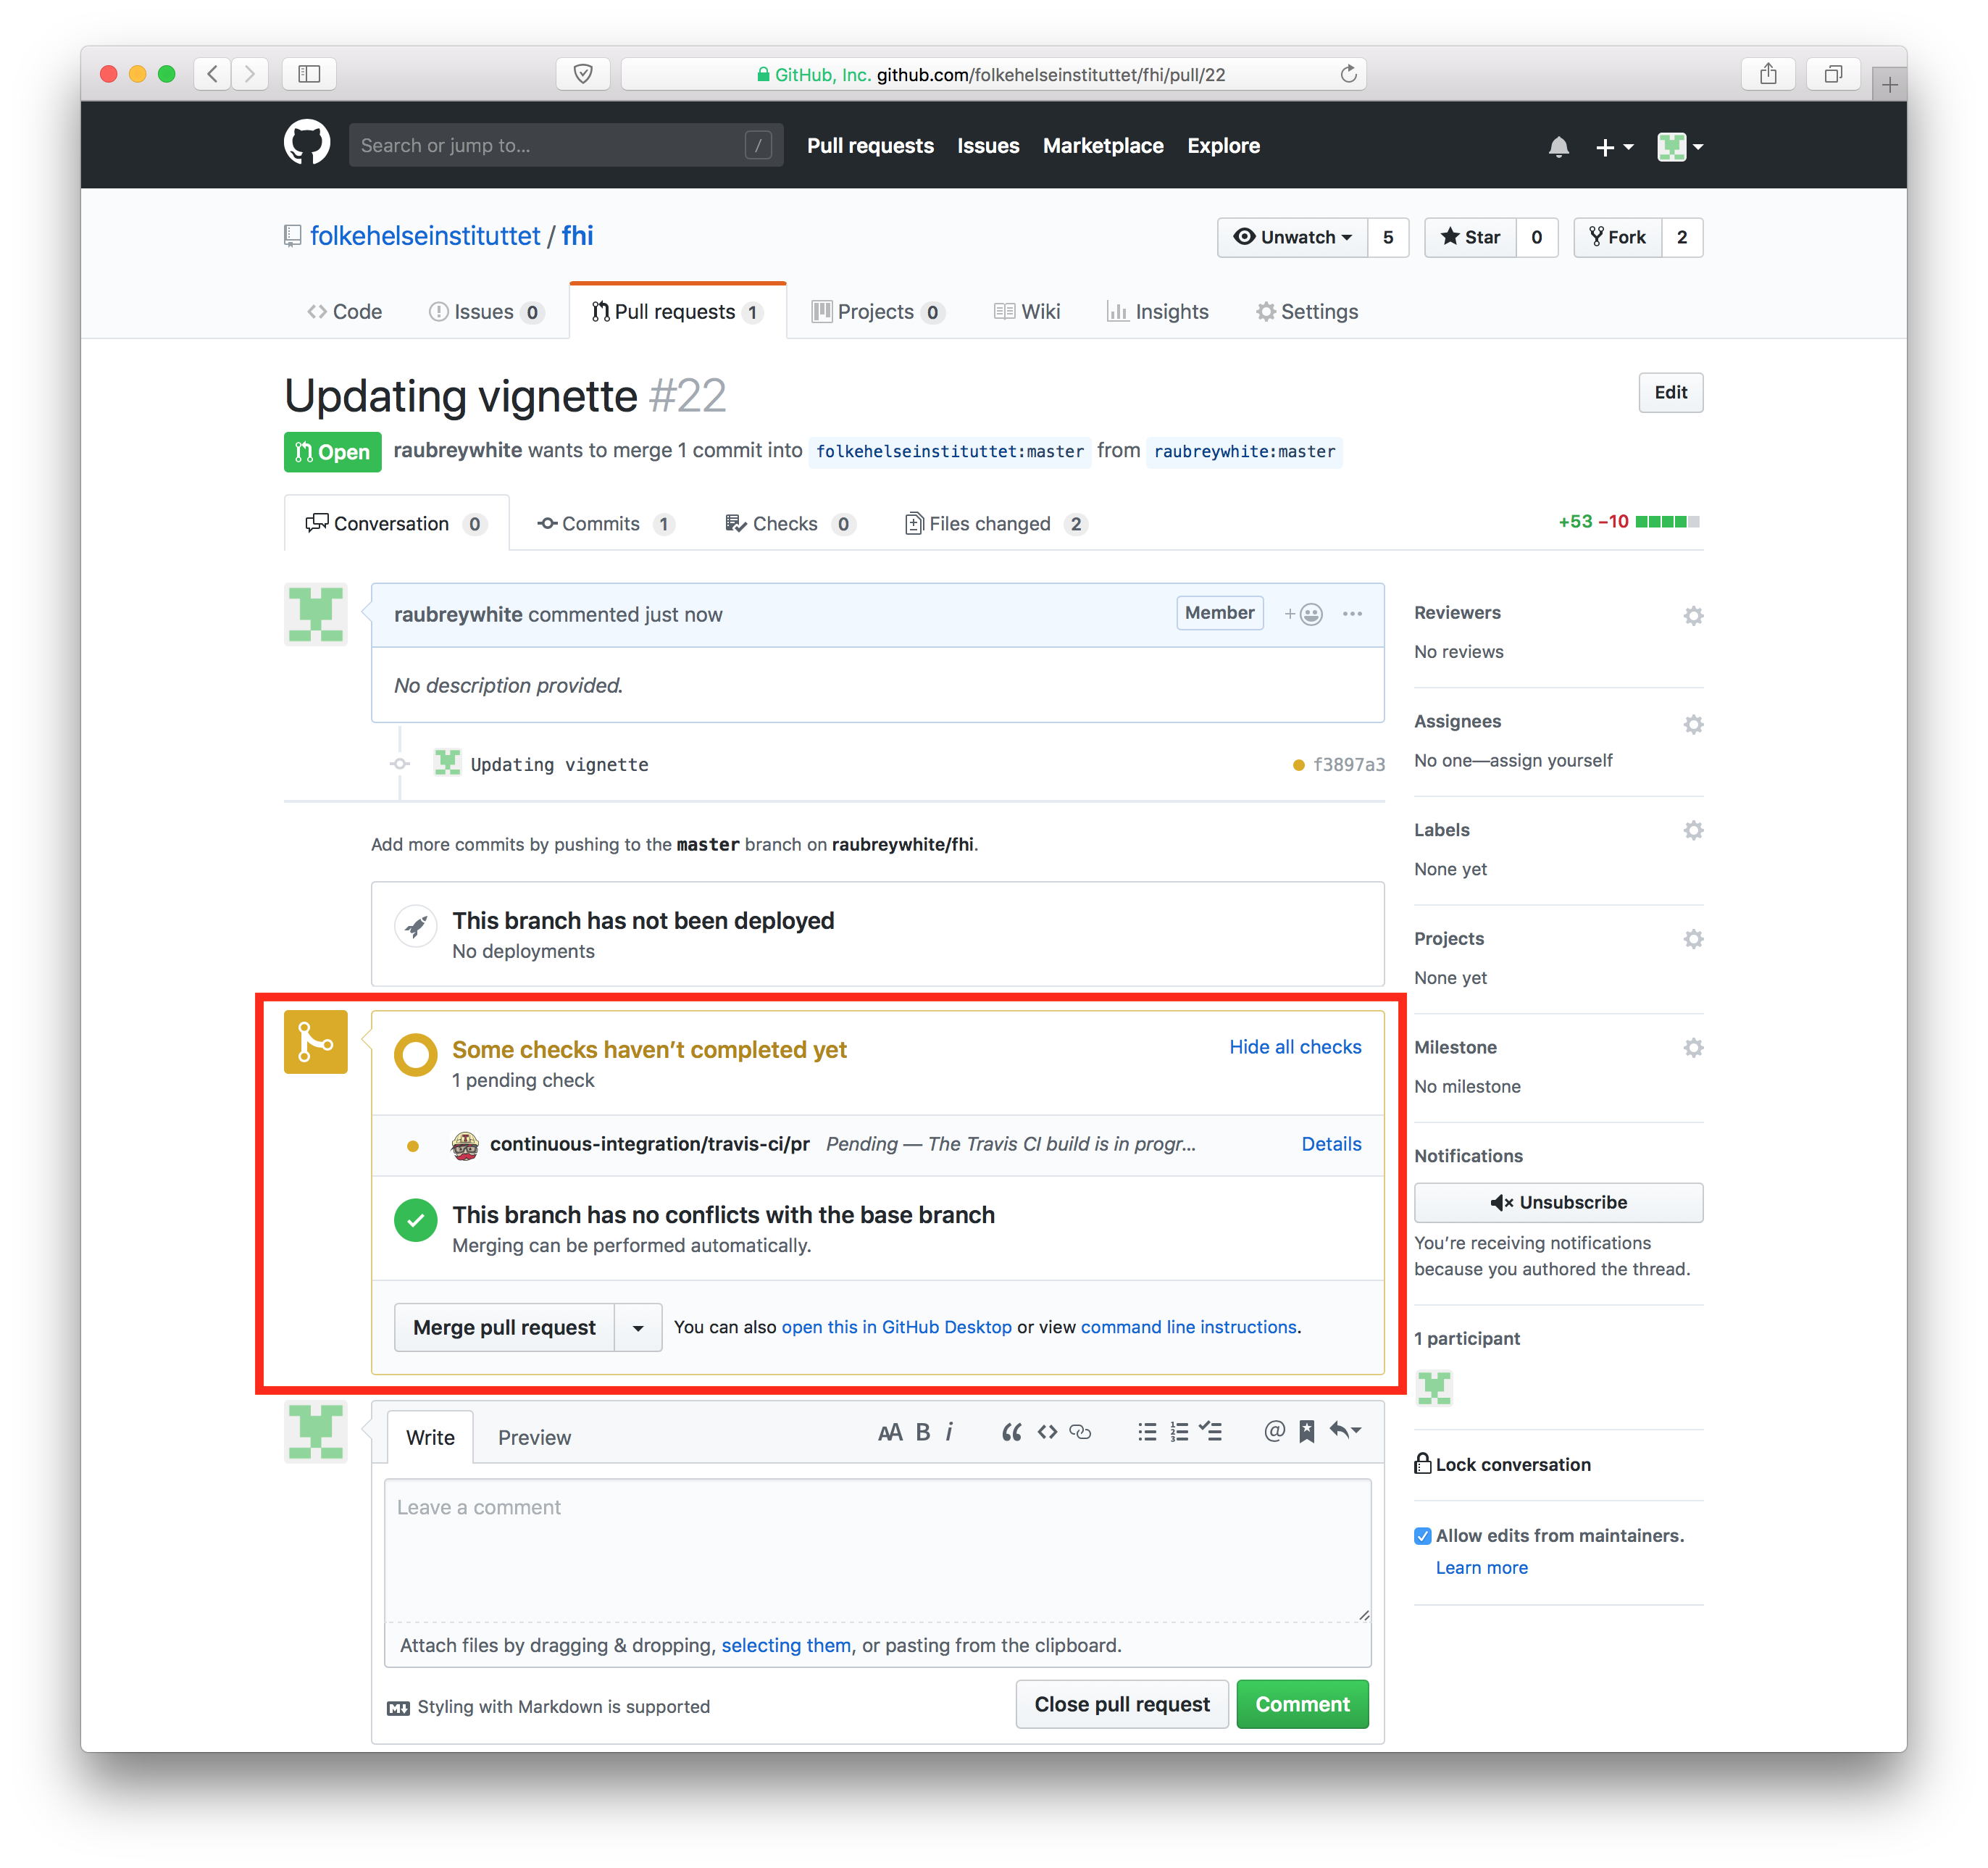
\includegraphics{images/pull_request_before_checks.png}

\begin{enumerate}
\def\labelenumi{\arabic{enumi}.}
\setcounter{enumi}{8}
\tightlist
\item
  Please make sure that the unit tests \texttt{PASS} before merging in!!
\end{enumerate}

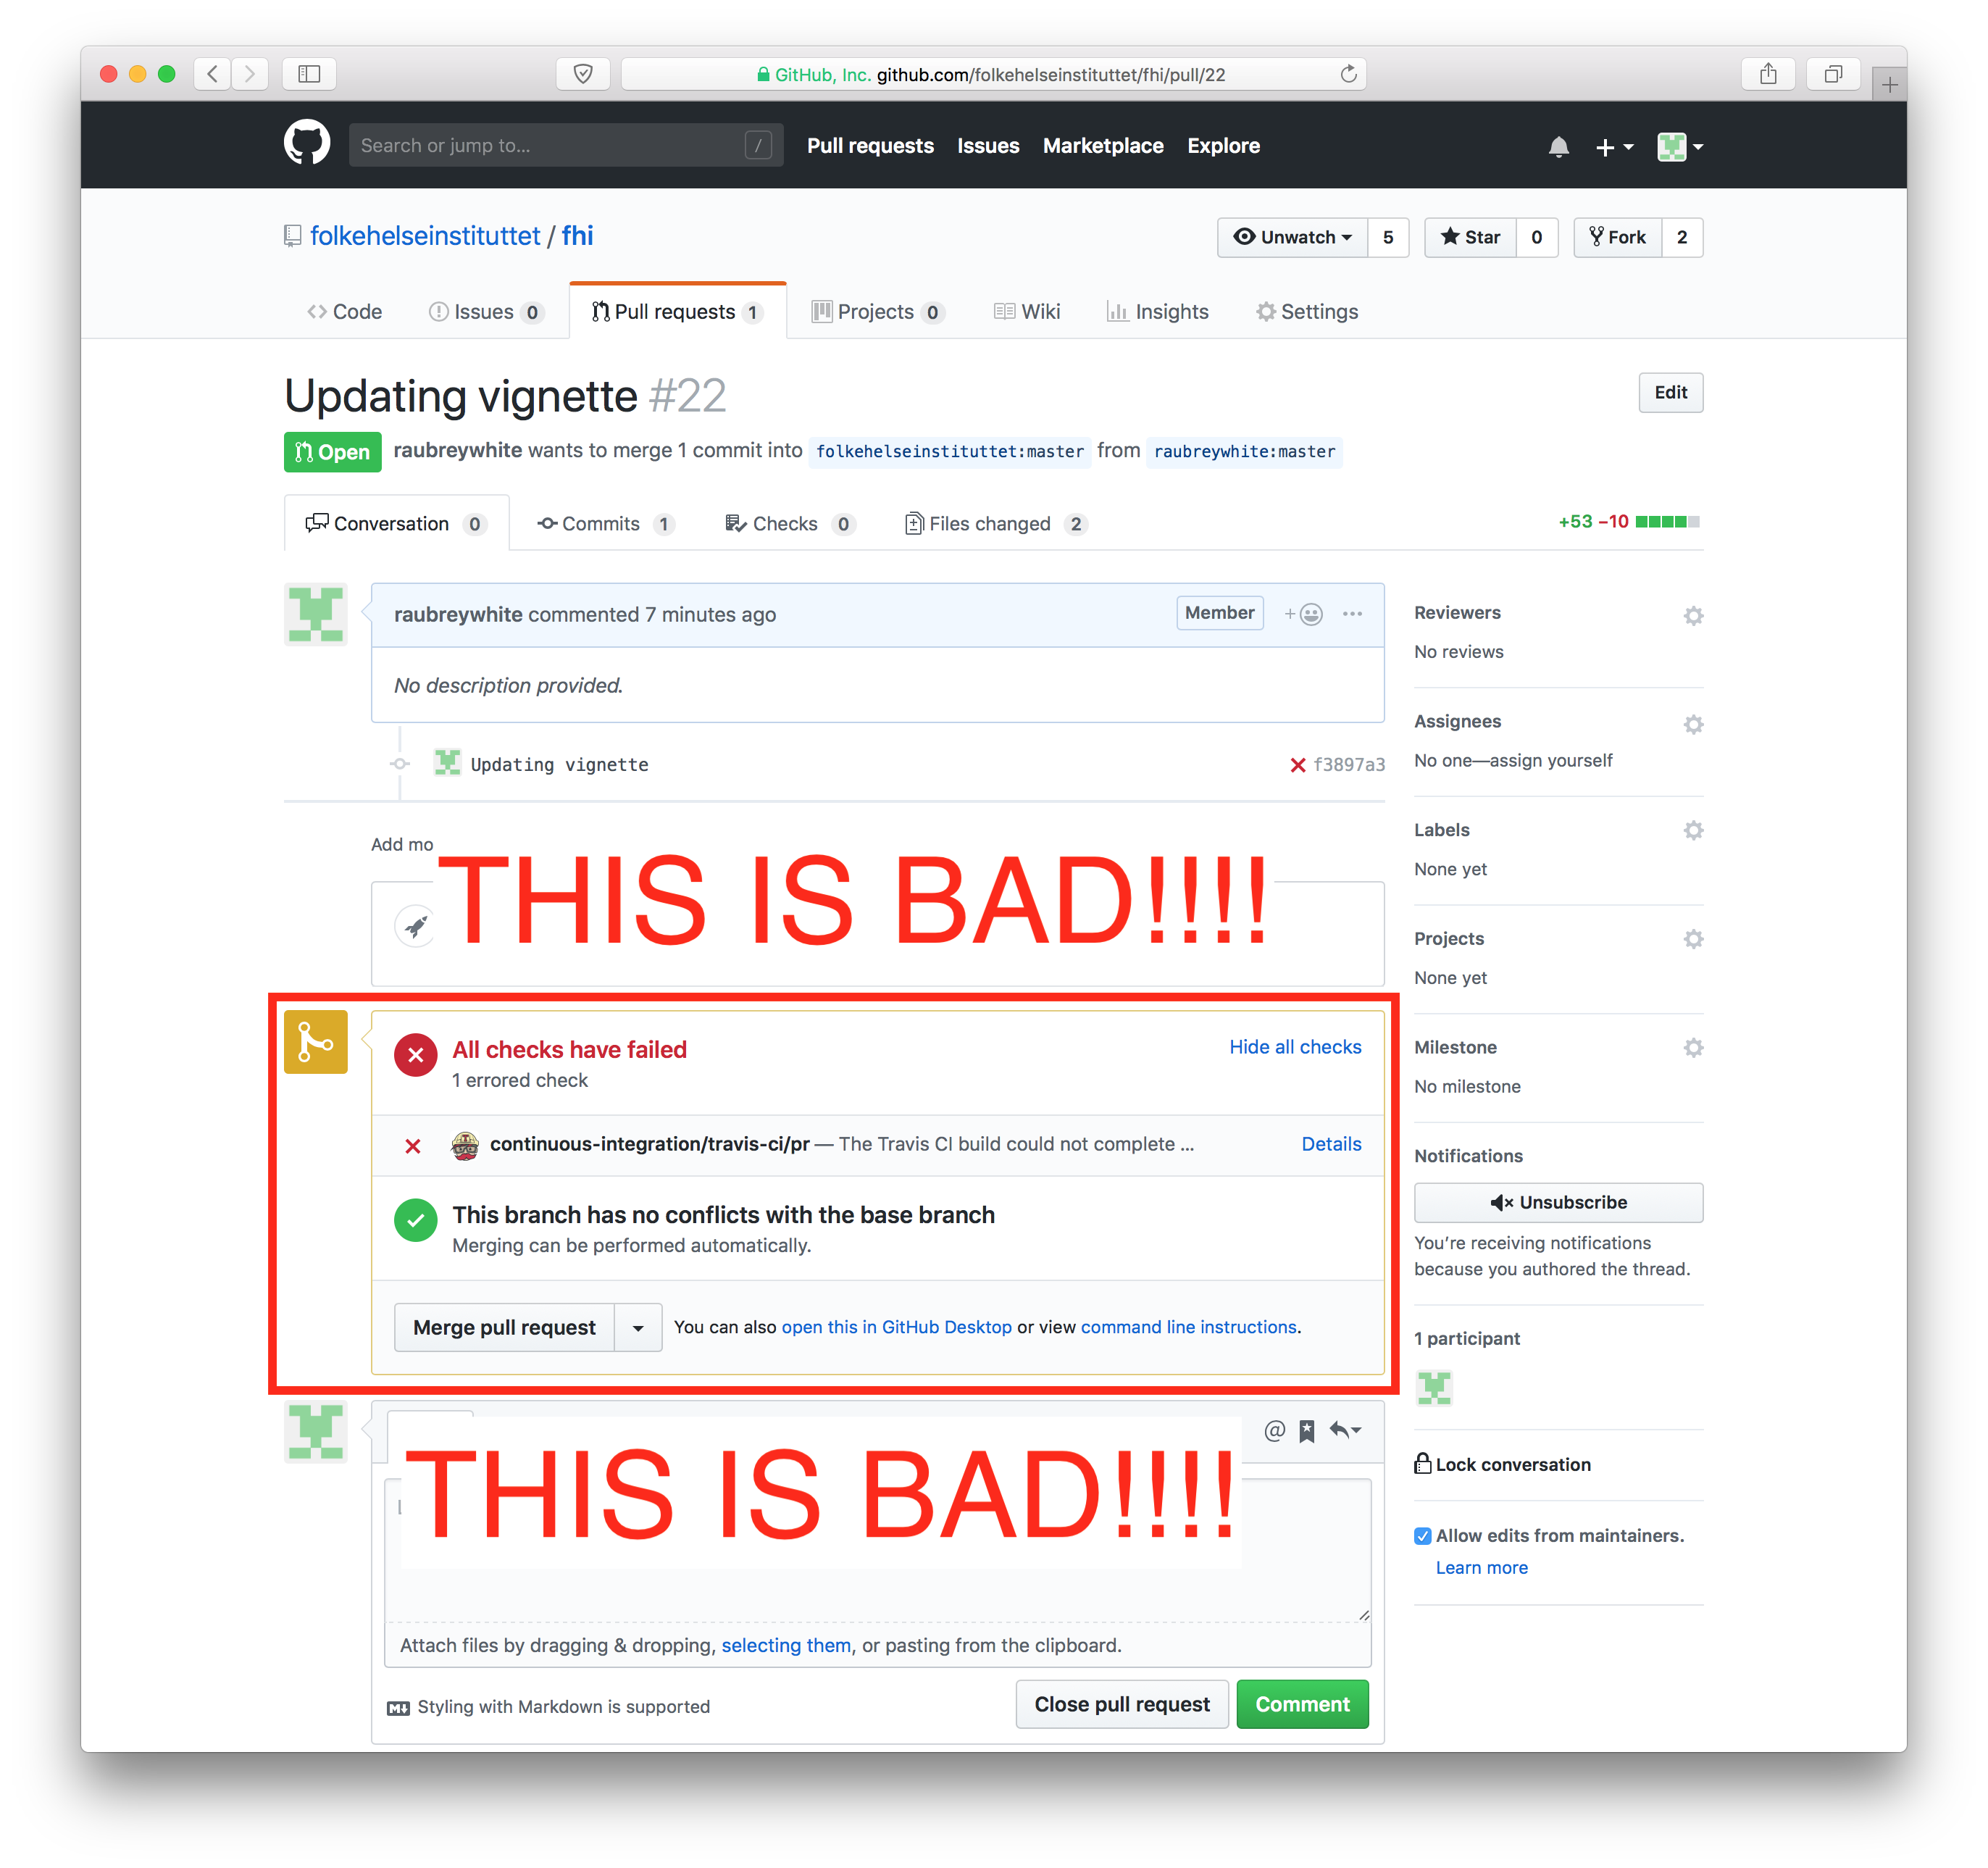
\includegraphics{images/pull_request_checks_failed.png}

\subsection{Code style}\label{code-style}

\begin{itemize}
\item
  Function names start with capital letters
\item
  Variable names start with small letters
\item
  Environments should be in ALL CAPS
\item
  Reference \href{http://adv-r.had.co.nz/Style.html}{Hadley's style
  code}
\item
  \textless{}- is preferred over = for assignment
\item
  Indentation is with two spaces, not two or a tab. There should be no
  tabs in code files.
\item
  if () \{\} else \{\} constructions should always use full curly braces
  even when usage seems unnecessary from a clarity perspective.
\item
  TODO statements should be opened as GitHub issues with links to
  specific code files and code lines, rather than written inline.
\item
  Follow Hadley's suggestion for aligning long functions with many
  arguments:

\begin{verbatim}
 long_function_name <- function(a = "a long argument", 
                            b = "another argument",
                            c = "another long argument") {
   # As usual code is indented by two spaces.
 }
\end{verbatim}
\item
  Never use print() to send text to the console. Instead use message(),
  warning(), and error() as appropriate.
\item
  Use environment variables, not options(), to store global arguments
  that are used by many or all functions.
\end{itemize}

\bibliography{book.bib}


\end{document}
